\section{Conclusion}
From the experimental results, we can conclude that given a constant size 9x9 median filter. Threading provides a significant improvement in performance. However, this improvement is not linear and simply adding K more threads to the problem will not give K performance gain.
\newline
No critical section needs to be considered in this case as the threads act independently to one another.
\newline
In selecting thread counts, it is best to match the number of execution cores (Physical + Logical) your system has. Any more threads adds minimal gain and in certain cases can lead to degradation in performance.
\newline
Data partitioning was shown to only produce improvements if the partitioning is done intelligently to ensure that each thread receives equal amounts of work to do. Badly portioning data can lead to some thread finishing early and this leads to wasted time. It also resolves to being algorithm specific.
\newline
In terms of golden-measure improvements and a fixed 9x9 mask size. The most optimal sort to use is the std::sort with 4 threads. This was shown to produce a speed up of 3.6x on average.
\newline
Further investigation should be done into the timing of functions by running the experiments in a perfectly unobstructed system with no system cache and only the mandatory minimum background processes running (Systemd, etc). Experiments should also be conducted with varying filter
 sizes.\\

Ailsa is a bad ass bitch\\
\begin{figure}[!]
	\centering
	
\includegraphics[scale=0.8]{Figures/small.jpg}
	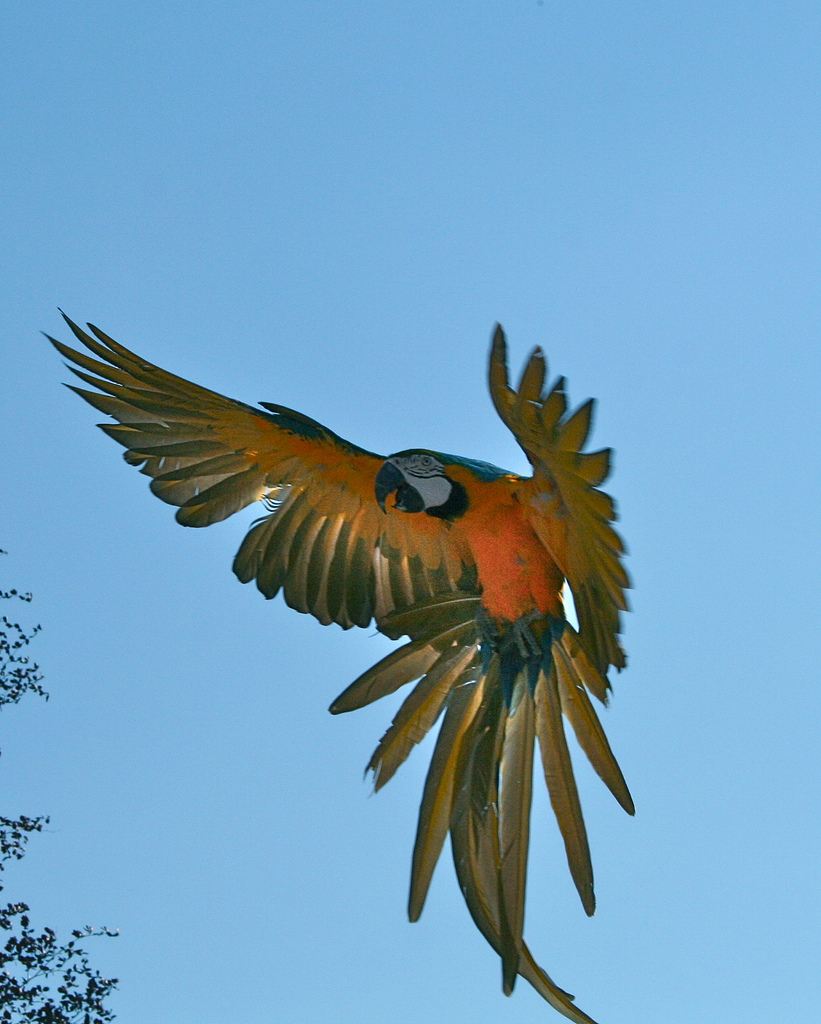
\includegraphics[scale=0.07]{Figures/fly.jpg}
	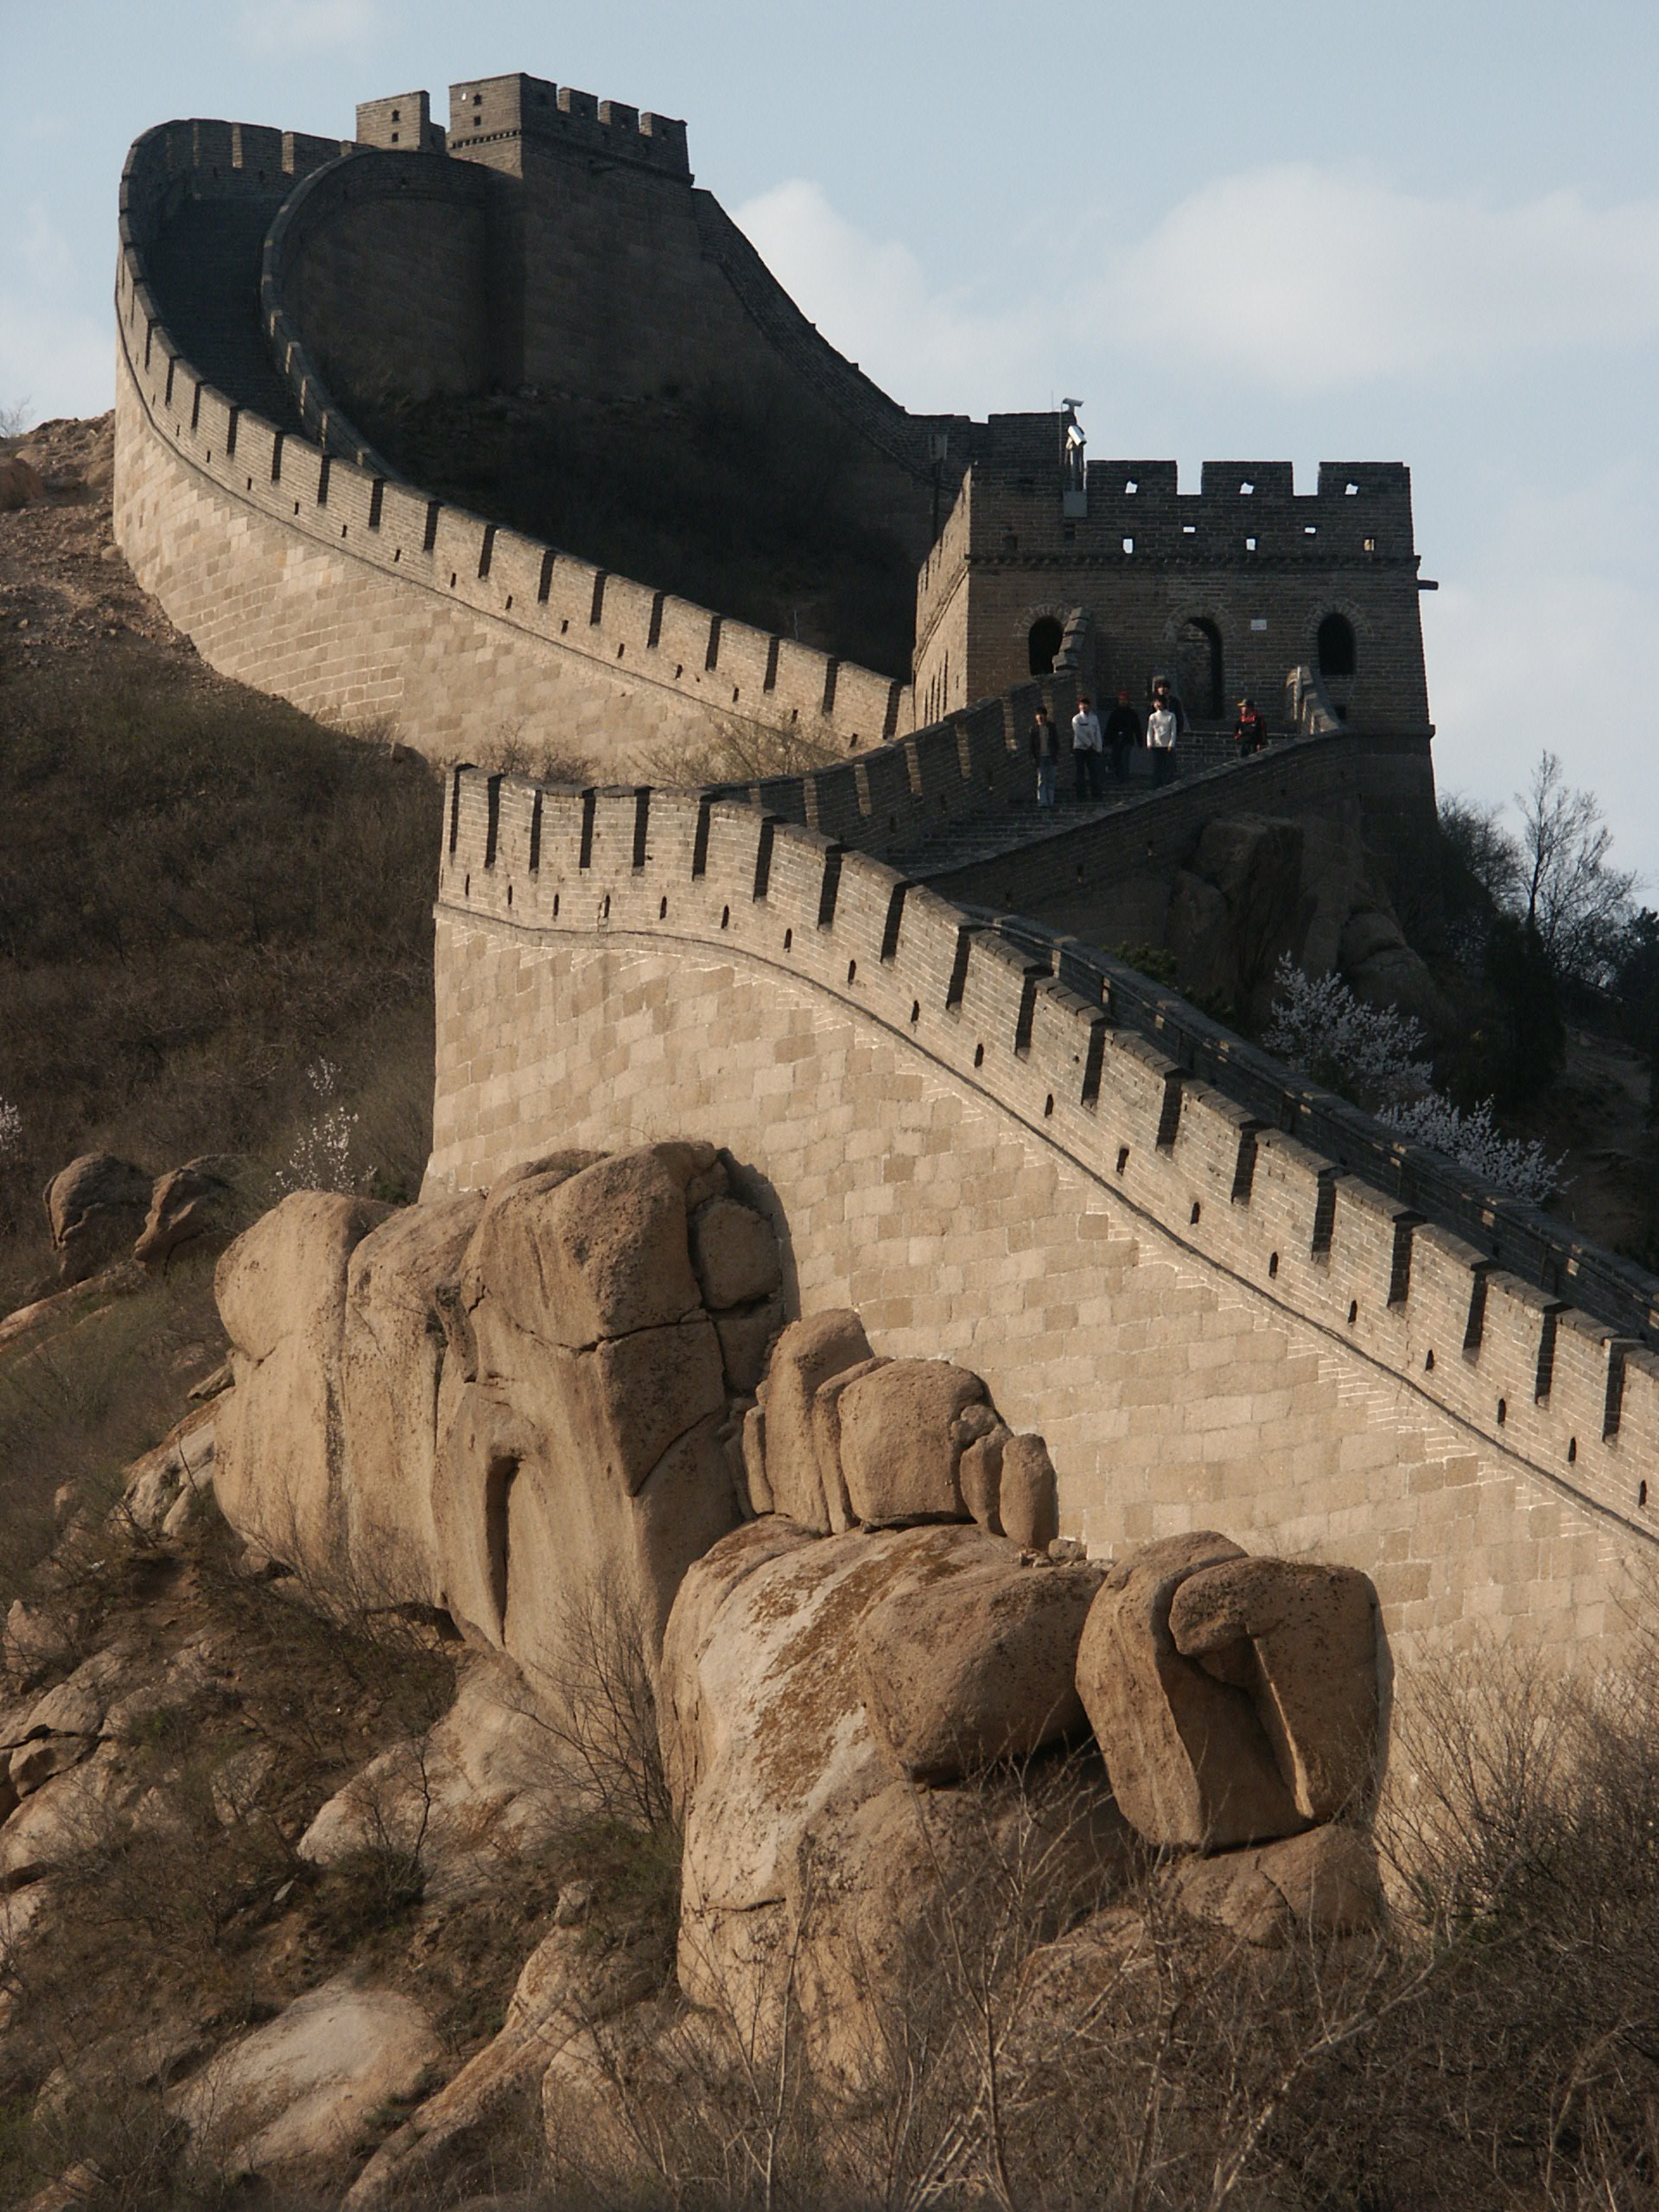
\includegraphics[scale=0.04]{Figures/greatwall.jpg}
	
\includegraphics[scale=0.04]{Figures/place.jpg}	
    \caption{Sample Input Images}
	\label{tss}
\end{figure}
\begin{figure}[!]
	\centering
	
\includegraphics[scale=0.2]{Figures/smallO.jpg}
	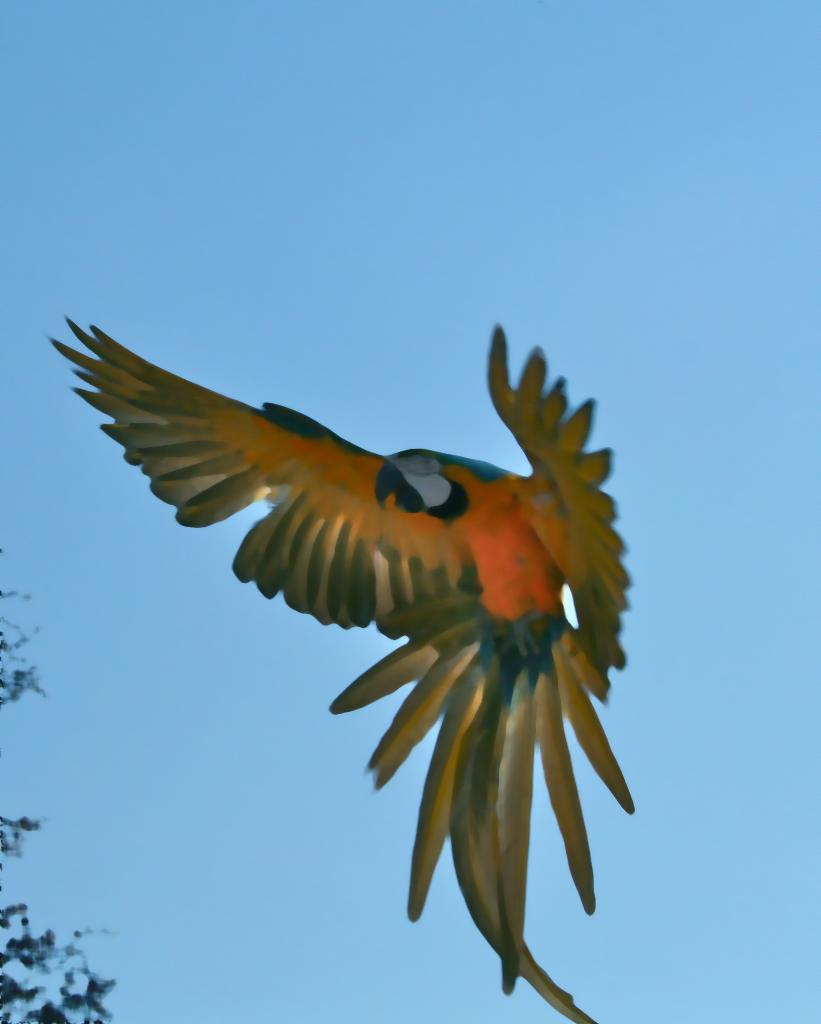
\includegraphics[scale=0.07]{Figures/flyO.jpg}
	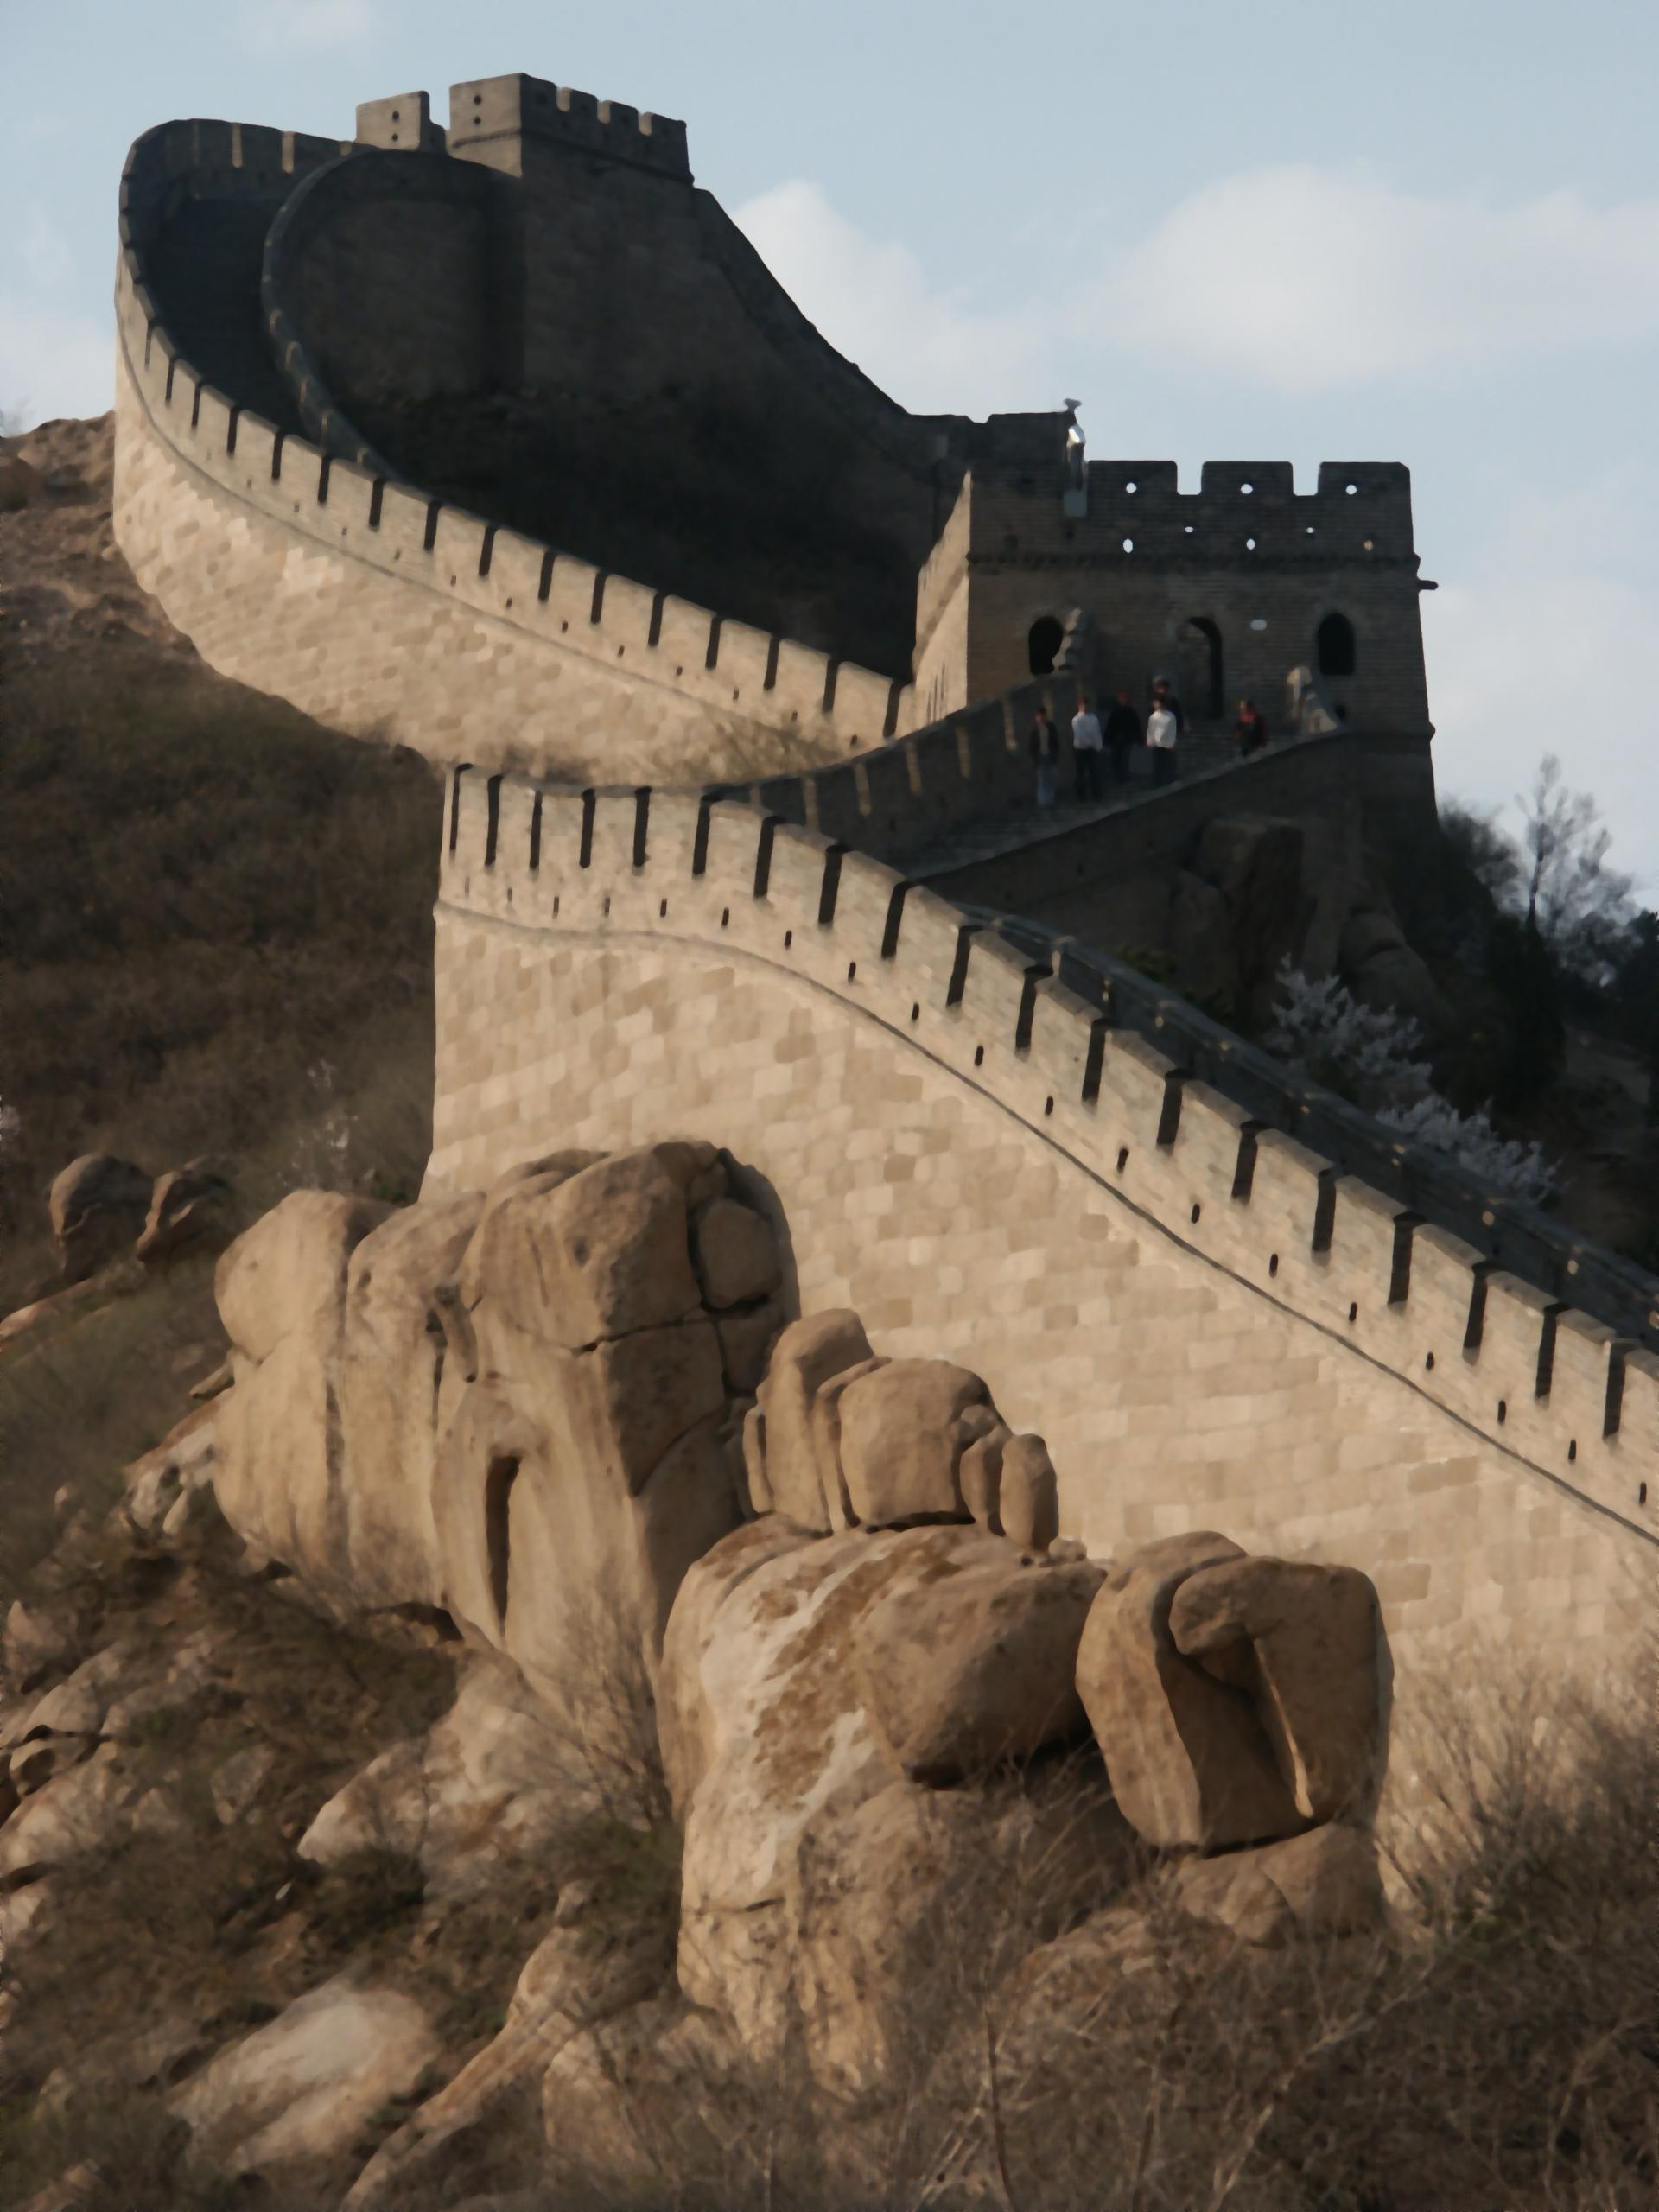
\includegraphics[scale=0.04]{Figures/greatwallO.jpg}
	
\includegraphics[scale=0.04]{Figures/placeO.jpg}	
    \caption{Sample Output Images}
	\label{tss}
\end{figure}